\usetikzlibrary{calc,positioning}
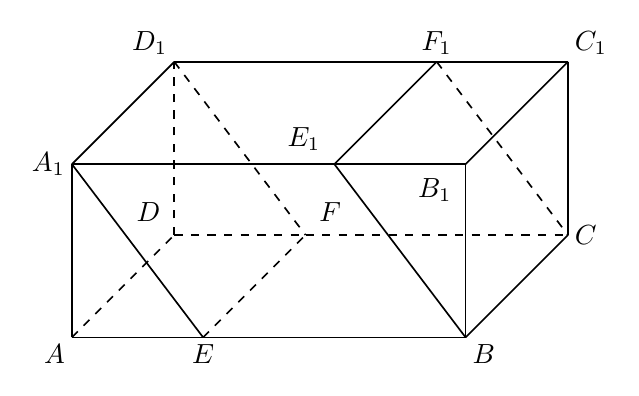
\begin{tikzpicture}[x=1cm,y=1cm,line width=.6pt,font=\normalsize,
 geometry edge/.style={solid,line width=.6pt,draw=black},
 geometry label/.style={font=\normalsize,inner sep=1.5pt,outer sep=1pt,draw=none}]

\coordinate (A) at (0,0);
\coordinate (E) at (1.666666667,0);
\coordinate (B) at (5.0,0);
\coordinate (A1) at (0,2.2);
\coordinate (E1) at (3.333333333,2.2);
\coordinate (B1) at (5.0,2.2);
\coordinate (D) at (1.3,1.3);
\coordinate (F) at (2.966666667,1.3);
\coordinate (C) at (6.3,1.3);
\coordinate (D1) at (1.3,3.5);
\coordinate (F1) at (4.633333333,3.5);
\coordinate (C1) at (6.3,3.5);
\draw[geometry edge] (A)--(B);
\draw[geometry edge] (A)--(A1);
\draw[geometry edge] (A1)--(B1);
\draw[geometry edge] (B)--(B1);
\draw[geometry edge] (A1)--(E);
\draw[geometry edge] (E1)--(B);
\draw[geometry edge] (A1)--(D1);
\draw[geometry edge] (D1)--(C1);
\draw[geometry edge] (F1)--(E1);
\draw[geometry edge] (B1)--(C1);
% hidden edge C1-C drawn dashed below
% B-C hidden: no visible stroke in original
\draw[geometry edge,dashed] (A)--(D);
\draw[geometry edge,dashed] (D)--(F);
\draw[geometry edge,dashed] (F)--(C);
\draw[geometry edge,dashed] (D)--(D1);
\draw[geometry edge,dashed] (D1)--(F);
\draw[geometry edge,dashed] (E)--(F);
\draw[geometry edge,dashed] (F1)--(C);
\draw[geometry edge] (C1)--(C) (B)--(C);
\node[geometry label,below left] at (A) {$A$};
\node[geometry label,below] at (E) {$E$};
\node[geometry label,below right] at (B) {$B$};
\node[geometry label,left] at (A1) {$A_{1}$};
\node[above left=2pt] at (E1) {$E_{1}$};
\node[below left=2pt] at (B1) {$B_{1}$};
\node[above left=2pt] at (D) {$D$};
\node[above right=2pt] at (F) {$F$};
\node[geometry label,right] at (C) {$C$};
\node[geometry label,above left] at (D1) {$D_{1}$};
\node[geometry label,above] at (F1) {$F_{1}$};
\node[geometry label,above right] at (C1) {$C_{1}$};
\end{tikzpicture}
